\documentclass[a4paper,11pt]{article}
\usepackage{graphicx}
\usepackage{esvect}
\usepackage{subcaption}
\usepackage{listings}
\usepackage[top=0.75in, bottom=0.75in, left=0.6in, right=0.6in]{geometry}

\title{AE 625 - Particles Methods for Fluid Flow Simulation \\ Flow past circular cylinder with the RVM}
\author{Chillapalli Jyothi Durga Prasad - 140010042 }
\date{21 August 2017}

\usepackage{color}
 

\begin{document}
\maketitle


\tableofcontents
\listoffigures


\newpage
\section*{Using the Runge-Kutta integrator and the linear vortex panel method to simulate the flow past a circular cylinder of unit radius (R; D = 2R) centered at the origin at a Reynolds number ($Re = U D/\nu$) of 1000. Use the RVM for diffusion and use Chorin blobs.}

\indent The cylinder can be stationary with a constant free-stream. Choose $\gamma$max=0.1 and use anywhere between 25 to 75 panels for the body. Simulate this problem for a time of at least 3 seconds in total (ideally 4-5 seconds). Use a $\delta$t between 0.05 and 0.1 (0.1 is perfectly OK). Increase $\gamma$max if your code takes too long to run. Calculate the vortex momentum for the simulation.\\

Re = 1000 ; U = 1 m/s; D = 2 m; $\nu$ = UD/Re\\

The algorithm used for the following simulations:\\

\begin{centering}
\begin{itemize}
  \item Solve Linear Vortex Panel Method for free stream.\\
  \item Introduce vortex particles to nullify slip over the panels. \\
  \item Convect the vortex particles in the stream using RK2 time integration.\\
  \item Check for penetration of vortex blobs with body and reflect them.\\
  \item Diffuse all vortex particles\\
  \item Check for penetration of vortex blobs with body and reflect them.\\

\end{itemize}
\end{centering}

\newpage

\section{Plot tte vortices at each second (1, 2, ... 5), color the positive blobs differently from the negative ones.}

\textbf{Results:}\\


\begin{figure}[ht]
    \centering
    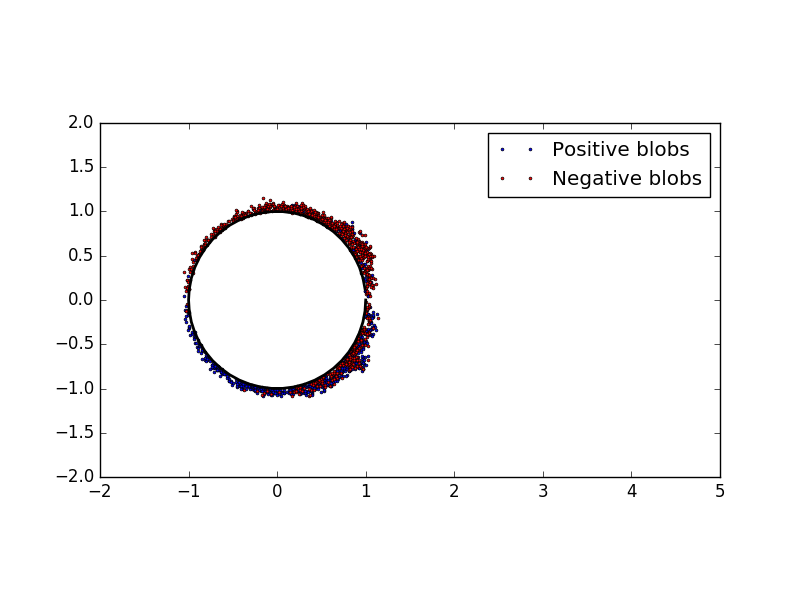
\includegraphics[width=.8\linewidth]{rb_1.png}
    \caption{vortex particles after 1 sec}
    \label{fig:ex}    
\end{figure}

\begin{figure}[ht]
	\centering
	\begin{subfigure}[ht]{.5\textwidth}
  		\centering
  		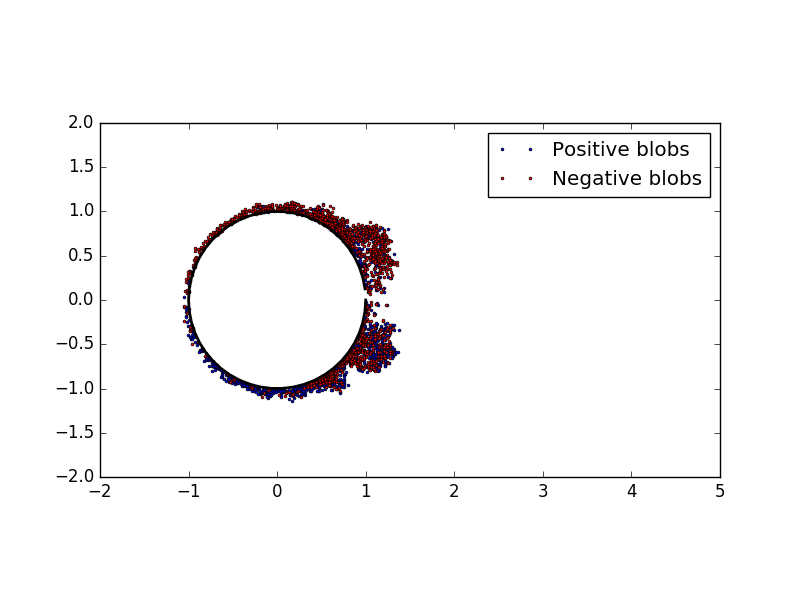
\includegraphics[width=.8\linewidth]{rb_2.png}
  		\caption{vortex particles after 2 sec}
  		\label{fig:16}
	\end{subfigure}
	\begin{subfigure}[ht]{.5\textwidth}
  		\centering
  		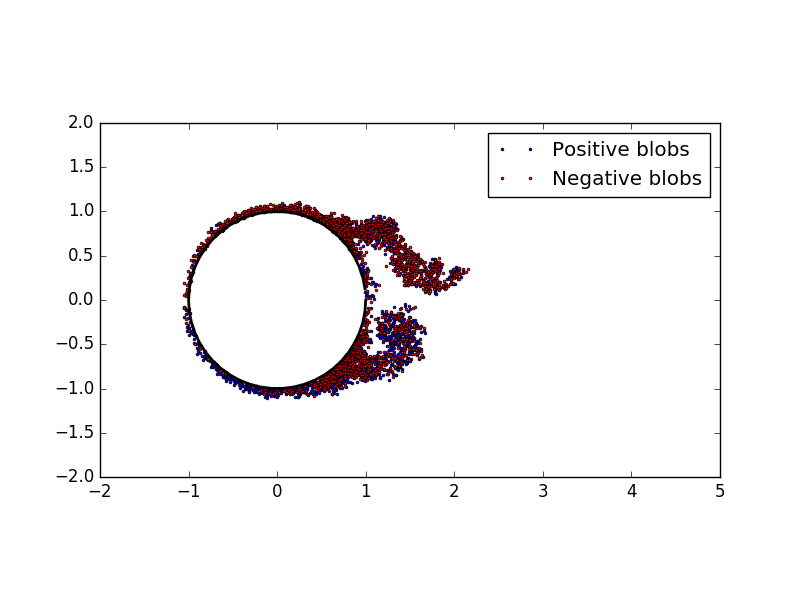
\includegraphics[width=.8\linewidth]{rb_3.png}
  		\caption{vortex particles after 3 sec}
  		\label{fig:25}
	\end{subfigure}%
	\label{fig:Question 1a}
  \caption{vortex particles after 2 and 3 sec}
\end{figure}

\begin{figure}[ht]
	\centering
	\begin{subfigure}[ht]{.5\textwidth}
  		\centering
  		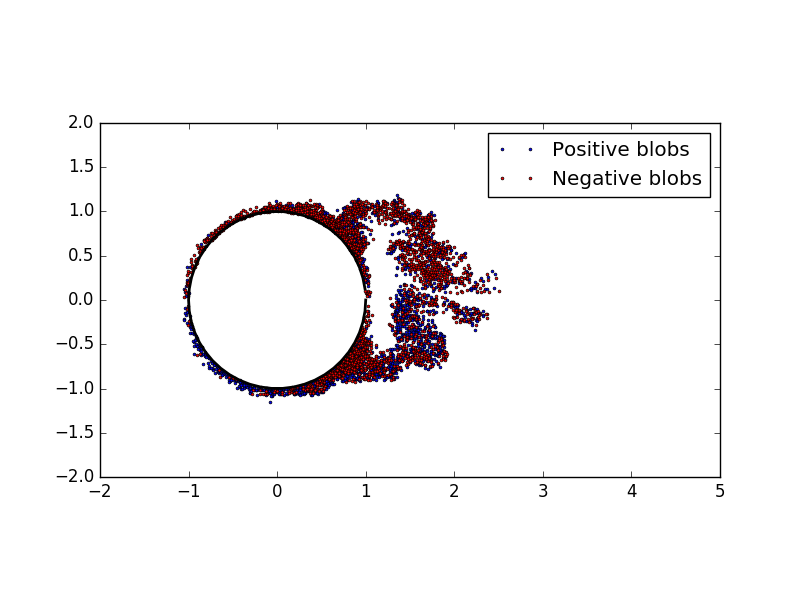
\includegraphics[width=.8\linewidth]{rb_4.png}
  		\caption{vortex particles after 4 sec}
  		\label{fig:36}
	\end{subfigure}
	\begin{subfigure}[ht]{.5\textwidth}
  		\centering
  		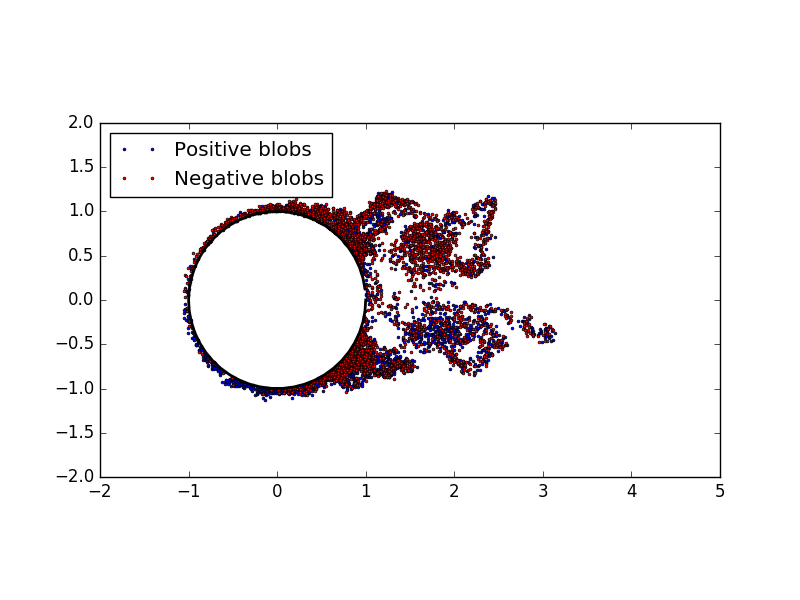
\includegraphics[width=.8\linewidth]{rb_5.png}
  		\caption{vortex particles after 5 sec}
  		\label{fig:49}
	\end{subfigure}%
	\label{fig:Question 1a}
  \caption{vortex particles after 4 and 5 sec}
\end{figure}

\begin{figure}[ht]
	\centering
	\begin{subfigure}[ht]{.5\textwidth}
  		\centering
  		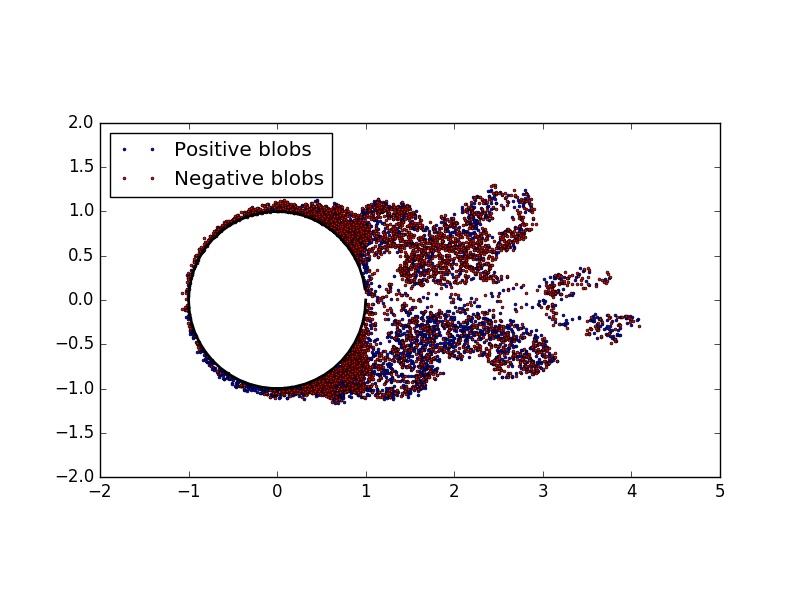
\includegraphics[width=.8\linewidth]{rb_7.png}
  		\caption{vortex particles after 7 sec}
  		\label{fig:64}
	\end{subfigure}
	\begin{subfigure}[ht]{.5\textwidth}
  		\centering
  		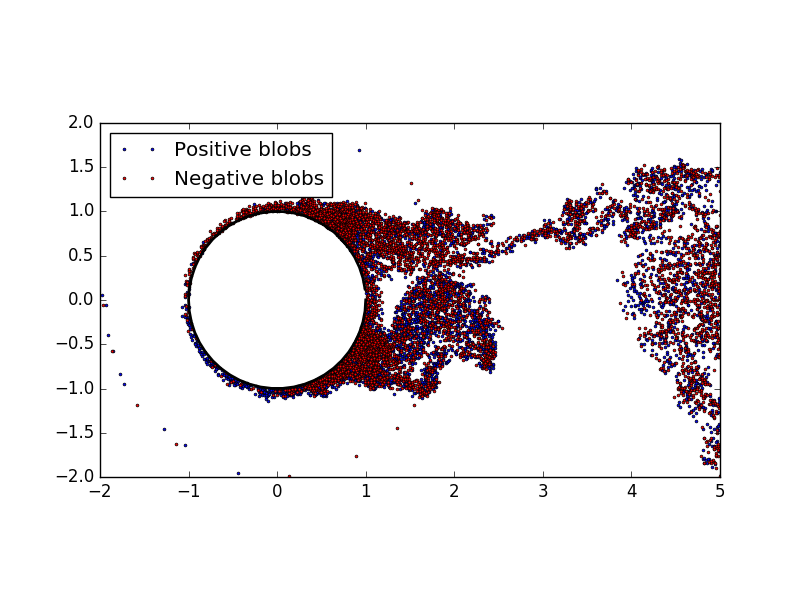
\includegraphics[width=.8\linewidth]{rb_15.png}
  		\caption{vortex particles after 15 sec}
  		\label{fig:80}
	\end{subfigure}
	\label{fig:Question 1a}
  \caption{vortex particles after 7 and 15 sec}
\end{figure}

\newpage
\indent\\
\newpage
\indent\\
\newpage
\indent\\
\section{Plot the velocity field around the cylinder at the final time (at least). Show the region (-2,-2) to (2,2) and also plot the region (0,0), (2,2) to show just the separated region.}

\textbf{Results:}

\indent The velocity field is as follows.
\begin{figure}[ht]
    \centering
    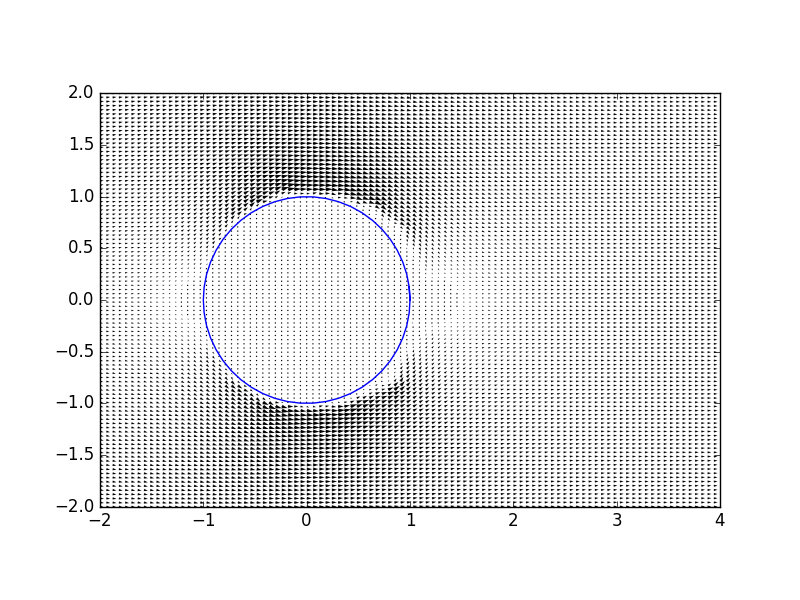
\includegraphics[width=.8\linewidth]{qui_1.png}
    \caption{velocity field after 1 sec}
    \label{fig:ex1}    
\end{figure}

\begin{figure}[ht]
  \centering
  \begin{subfigure}[ht]{.5\textwidth}
      \centering
      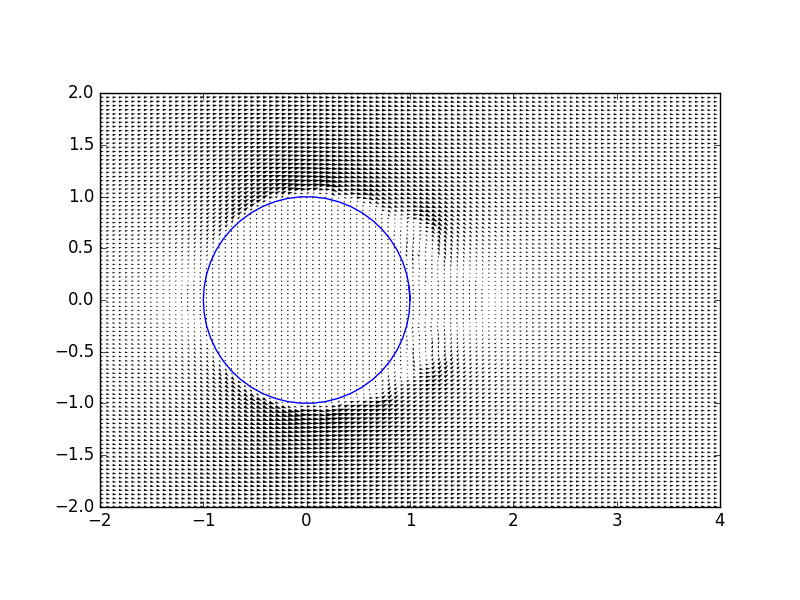
\includegraphics[width=.8\linewidth]{qui_2.png}
      \caption{velocity field after 2 sec}
      \label{fig:161}
  \end{subfigure}
  \begin{subfigure}[ht]{.5\textwidth}
      \centering
      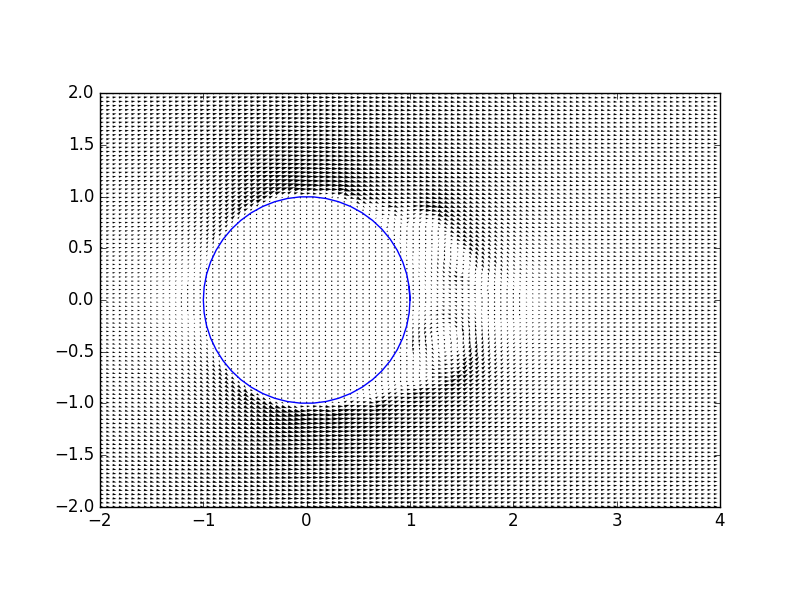
\includegraphics[width=.8\linewidth]{qui_3.png}
      \caption{velocity field after 3 sec}
      \label{fig:251}
  \end{subfigure}%
  \label{fig:Question 1a1}
  \caption{velocity field after 2 and 3 sec}
\end{figure}

\begin{figure}[ht]
  \centering
  \begin{subfigure}[ht]{.5\textwidth}
      \centering
      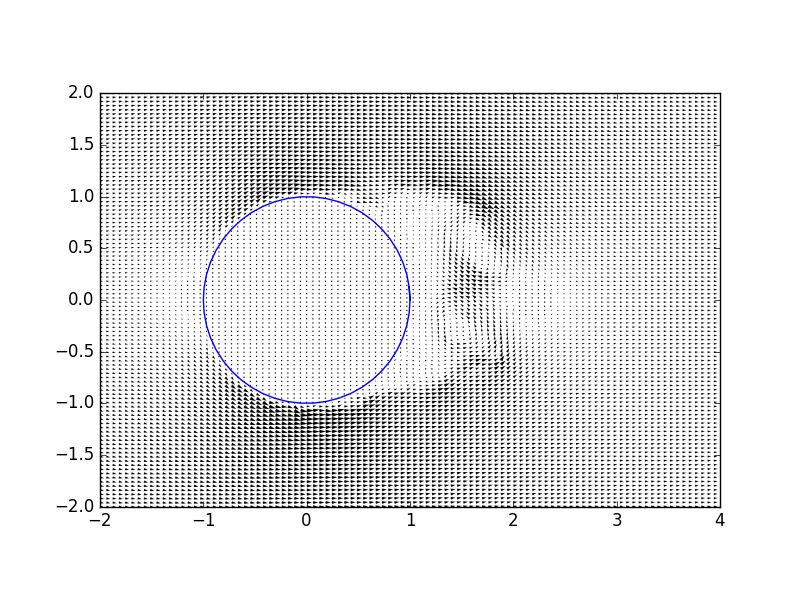
\includegraphics[width=.8\linewidth]{qui_4.png}
      \caption{velocity field after 4 sec}
      \label{fig:361}
  \end{subfigure}
  \begin{subfigure}[ht]{.5\textwidth}
      \centering
      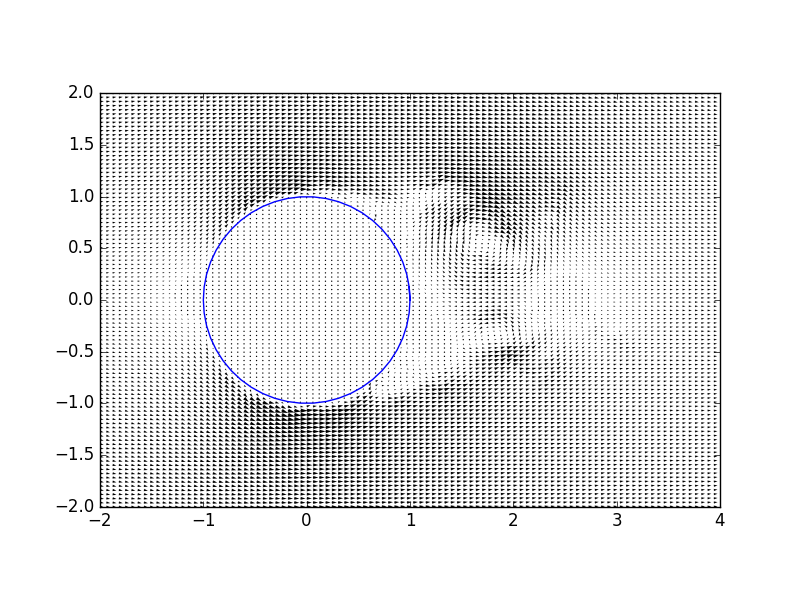
\includegraphics[width=.8\linewidth]{qui_5.png}
      \caption{velocity field after 5 sec}
      \label{fig:491}
  \end{subfigure}%
  \label{fig:Question 1a1}
  \caption{velocity field after 4 and 5 sec}
\end{figure}

\begin{figure}[ht]
  \centering
  \begin{subfigure}[ht]{.5\textwidth}
      \centering
      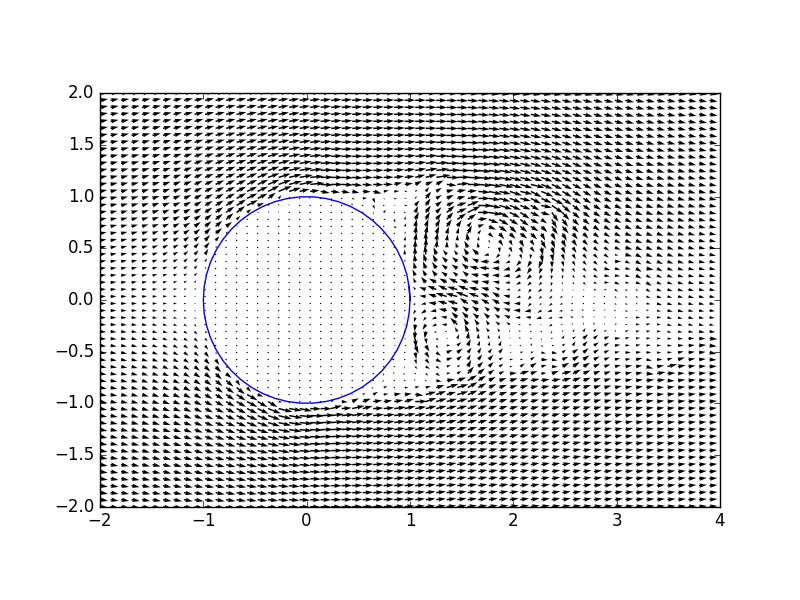
\includegraphics[width=.8\linewidth]{qui_7.png}
      \caption{velocity field after 7 sec}
      \label{fig:641}
  \end{subfigure}
  \begin{subfigure}[ht]{.5\textwidth}
      \centering
      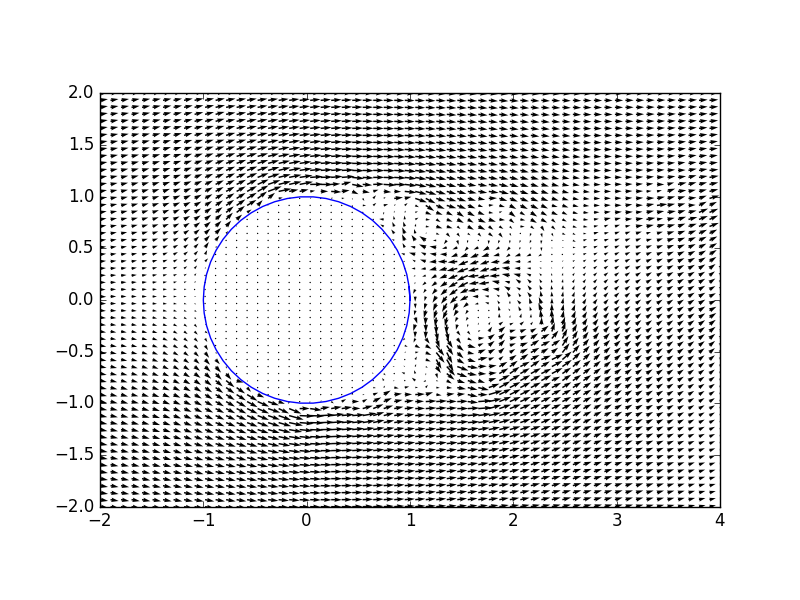
\includegraphics[width=.8\linewidth]{qui_15.png}
      \caption{velocity field after 15 sec}
      \label{fig:801}
  \end{subfigure}
  \label{fig:Question 1a1}
  \caption{velocity field after 7 and 15 sec}
\end{figure}
\indent the following shows the separated region for t = 5 sec\\

\begin{figure}[ht]
    \centering
    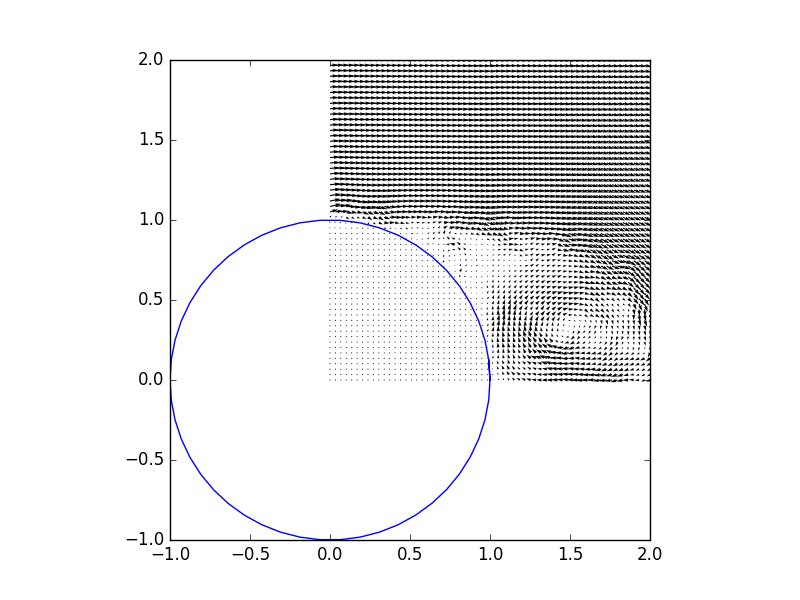
\includegraphics[width=.8\linewidth]{sep_reg_5.png}
    \caption{velocity field after 1 sec}
    \label{fig:ex2}    
\end{figure}

\newpage
\indent\\
\newpage
\indent\\
\newpage
\indent\\
\newpage
\indent\\
\newpage
\indent\\
\newpage
\indent\\

\section{Smooth the vortex momentum using running averages take the derivative and  plot $C_D$ vs time for the simulation.}

\textbf{Results:}\\

\indent $C_d$ and $C_l$ plots as follows.\\
$C_d$ and $C_l$ tend to ocscillate about 1 and 0 respectively for Re = 1000.\\ 

\begin{figure}[ht]
    \centering
    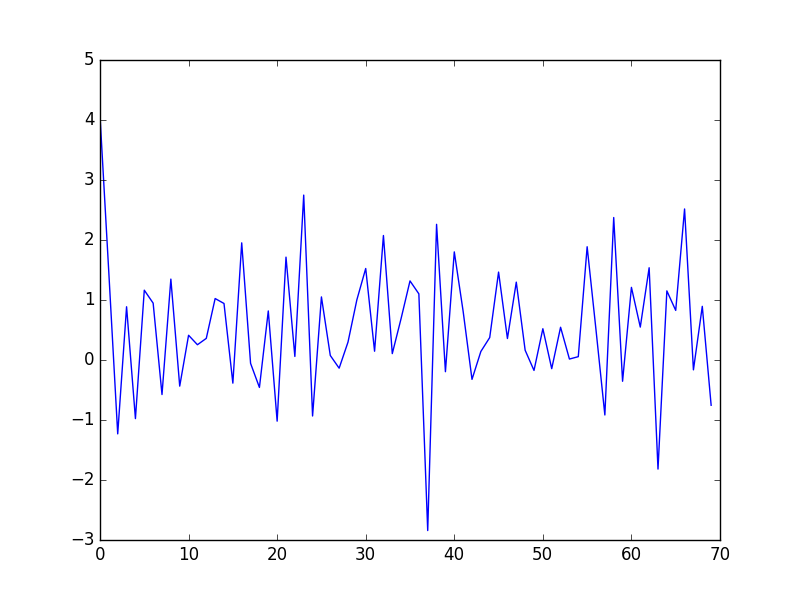
\includegraphics[width=.8\linewidth]{cd_re1000.png}
    \caption{Cd caluclated with running average of vortex momentum.}
    \label{fig:cd}    
\end{figure}

\begin{figure}[ht]
    \centering
    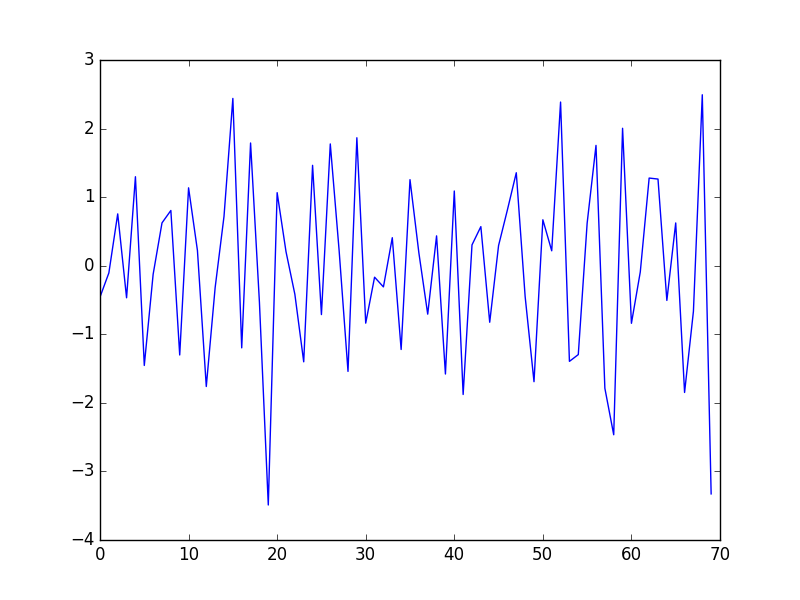
\includegraphics[width=.8\linewidth]{Cl_re1000.png}
    \caption{Cl caluclated with running average of vortex momentum.}
    \label{fig:cl}    
\end{figure}

\end{document}

